% File Name: Saurav_Kumar_Resume.tex
% Description: LaTeX code for Resume
% Author: Saurav Kumar
% Created: 17 April 2019, 08:40 aM

\documentclass[11pt]{article}

% Import Packages
\usepackage{graphicx}
\usepackage[none]{hyphenat}
\usepackage{array}
\usepackage[parfill]{parskip}
\usepackage{titlesec}
\usepackage{titling}
\usepackage{microtype}
\usepackage{vwcol}  
\usepackage[a4paper, margin=1.5cm]{geometry}
\usepackage[sfdefault, medium]{roboto}
\usepackage[T1]{fontenc}
\usepackage{enumitem}

% Format Sections
\titleformat{\section}
{\LARGE}
{}
{0cm}
{\bfseries\lowercase}[\titlerule]

% ---------- Begin Document ----------
\begin{document}

% Title
\begin{center}
\fontsize{30pt}{18pt}
\fontseries{b}\selectfont Saurav 
\fontseries{l}\selectfont Kumar\\
\fontsize{16pt}{28pt}\fontseries{l}\selectfont R \'{e} s u m \'{e}
\end{center}
\vspace{1cm}

\begin{vwcol}[widths={0.235,0.6}, sep=1.3cm, justify=flush, rule=0.1pt, indent=0em] 
% ---------- Side Bar ----------
% Photo
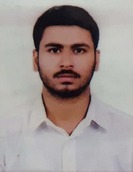
\includegraphics[scale=0.012]{saurav.jpg}
\vspace{0.3cm}

% Personal Details
\fontsize{15.5pt}{18pt}\selectfont
\mdseries personal \bfseries details
\rule{3.9cm}{0.1pt}

% Contact
\fontsize{11.5pt}{14pt}\selectfont
\fontseries{l}\selectfont Phone\\ 
\bfseries\selectfont +91 9915847709\vspace{1mm}

% Email ID
\rule{3.9cm}{0.1pt}\\ 
\fontseries{l}\selectfont Email ID\\ 
\bfseries\selectfont sauravgalaxy64@gmail\\
.com\\

% DOB
\rule{3.9cm}{0.1pt}\\
\fontseries{l}\selectfont Date of Birth\\ 
\bfseries\selectfont December 05, 1998\vspace{1mm}

% Gender
\rule{3.9cm}{0.1pt}\\
\fontseries{l}\selectfont Gender\\ 
\bfseries\selectfont Male\vspace{1mm}

% Nationality
\rule{3.9cm}{0.1pt}\\
\fontseries{l}\selectfont Nationality\\ 
\bfseries\selectfont Indian\vspace{1mm}

% Address
\rule{3.9cm}{0.1pt}\\
\fontseries{l}\selectfont Address\vspace{1.5mm}\\
\fontseries{m} \fontsize{10pt}{12pt} \selectfont
\begin{minipage}{3.9cm}
\bfseries\\H.NO: 2903/2 \\Sector 47-C,
 Chandigarh 160047, India\vspace{1mm}\\
\end{minipage}
\fontsize{11.5pt}{14pt}\selectfont

% Websites
\rule{3.9cm}{0.1pt}\\
\fontseries{l}\selectfont Websites\vspace{3mm}\\
\begin{tabular}{m{4mm}m{2cm}}

\includegraphics[scale=0.12]{github.png}&\bfseries\selectfont\textit{hacksaurav}\\
\includegraphics[scale=0.10]{linkedin.png}&\bfseries\selectfont\textit{in/saurav98}\\
\end{tabular}

% ---------- Main Column ----------
\newpage 
\mdseries\fontsize{10pt}{13pt}\selectfont
\begin{minipage}{12.73cm}

% Summary
\section{Career Objective}
 A third year Electronics and Communication student with a great passion and enthusiasm for development in the field of Robotics and Embedded Systems. I am extremely dedicated and hard working and seeking for Internship at e-Yantra, IITB.\\

% Education
\section{Education}
\begin{tabular}{ |p{1cm}||p{3cm}|p{3cm}|p{2cm}|p{2cm}|  }
 \hline
 
 \hline
 S.NO &Degree/ Eaxam(with Discipline)& University/ College/ Board &Year of Passing&Percentage of marks/ CPI\\
 \hline
 1. & BE(ECE) & UIET,panjab University &2020 &8.40\\
 \hline
 2. & Higher Secondary School(Class 12) & K.V.3BRD, AFS, Chandigarh,CBSE &2016 &88.60\%\\
 \hline
 3. & Secondary School(Class 10) & K.V.3BRD, AFS, Chandigarh,CBSE &2014 &95\%\\

 \hline
\end{tabular}

% Projects
\section{Projects}
\begin{enumerate}[leftmargin=*]
\item \bfseries Pick and Place Bot\\
\mdseries Built a Pick and Place Bot on the theme of thirsty crow In the E-yantra with the help of Path solving Algorithm and Augmented Reality. Based on the ATmega2560 microcontroller.\\

\item \bfseries Server based pollution monitoring system(IOT)\\
\mdseries  Developed a device which will be used to monitor the pollution level and the temperature of the particular site and update the information on the web page as well as on the Excel sheets.Also had mail and sms alerts. The advantage of using this device is that it is low cost ,easy to use compared to other devices in the market.\\

\item \bfseries CNC PLOTTER\\
\mdseries This project is based on designing a 2D- plotter which can plot any image or any script on a particular page. In this project first we have to do the hardware part which is designing of plotter and then we have to work on software part which is the generation of the G-code of the image which we want to plot.This can be further modified so to plot any script in our own handwriting.
Project Link: https://drive.google.com/folderview?id=1c1WKXYKnKe-JWh214p9ESyvSVbsgZGpb
\end{enumerate}
\end{minipage}

\begin{minipage}{12.73cm}\vspace{2mm}
\begin{enumerate}[leftmargin=*]
\setcounter{enumi}{3}


\item \bfseries Other Projects\\
\mdseries IoT based Home Automation using NodeMCU | Piezoelectric Based Shoes for Energy Harvesting and Wireless Transmission | Gesture Controlled Bot. 
\end{enumerate}
\end{minipage}
\end{vwcol}

% ---------- Next Page ----------
\pagebreak
\begin{minipage}{18cm}
\fontsize{10pt}{13pt}\selectfont



% Training
\section{Training}
\begin{itemize}[leftmargin=*]
\item \bfseries Professional Training \mdseries (Undergraduate level) in C programming | Institue name: FORTUNE INSTITUTE | Date: (03 June 2017 - 18 july 2017 ) | Key Skills Involved: C Programming.\\



\item \bfseries Online Training \mdseries in Internet of Things | Institute Name: Internshala | Date: (1 september 2018 - 28 september 2018) | Key Skills Involved: IOT, Python, Server\\
\end{itemize}

% Work Experience
\section{Work Experience \& Internships}
\begin{itemize}[leftmargin=*]
\item \bfseries Design Innovation Centre(DIC), UIET, PU \mdseries | Period: January 2019-Current | Mentor: Yajvender Pal Verma (Asstt. Professor) | Key Skills Involved: Electronics, Circuit Designing. | Position: Paid Intern.\\

\item \bfseries Telecommunication Lab, UIET, PU \mdseries | Intern - (June 2018 - July 2018) | Developed a Nodemcu based device which is used to monitor the pollution level of environment in the Panjab university campus .\\


\end{itemize}

% Research Publications
\section{Research Publications}
\begin{enumerate}[leftmargin=*]
\item \bfseries none\\
\end{enumerate}

% Technical Skills
\section{Technical Skills}
\begin{itemize}[leftmargin=*]
\item \bfseries Languages\\
Programming: \mdseries C, C++, Assembly | 
\bfseries Scripting: \mdseries Python | 
\bfseries Others: \mdseries HTML, CSS, \LaTeX\\

\item \bfseries Microcontrollers / Development Boards Knowledge\\
\mdseries ATmega Series (AVR), Arduino, Intel 8051, NodeMCU, GSM Module\\

\item \bfseries Software Knowledge\\
\mdseries Proficient in Arduino IDE, Blender, MATLAB, Atmel Studio, Keil uVision and Microsoft Office.\\

\item \bfseries Other Skills\\
\mdseries Augmented Reality, 3D printing.\\
\end{itemize}

% Soft Skills
\fontsize{10pt}{13pt}\selectfont
\section{Soft Skills}
\begin{enumerate}[leftmargin=*]
\item  I have a strong Work Ethic and I am Self-Motivated to complete the tasks through Hard Work, Dedication and Professionalism. I am a good Leader and have handled positions of Responsibility in the past, as well as, have been; a Collaborative, Efficient and Supportive; Team Member. I try my best to complete any Challenging task upto the Highest Standard, while managing my Time Optimally.\\

\item \bfseries Languages: 
Full Professional Proficiency \mdseries English and Hindi | \bfseries Limited Working Proficiency \mdseries Spanish (Still Learning) | \bfseries Native \mdseries Angika
\end{enumerate}

\end{minipage}


\end{document}